\subsection{Módulo de Gestión de Recursos e Inventario (INV)}

\begin{figure}[H]\centering
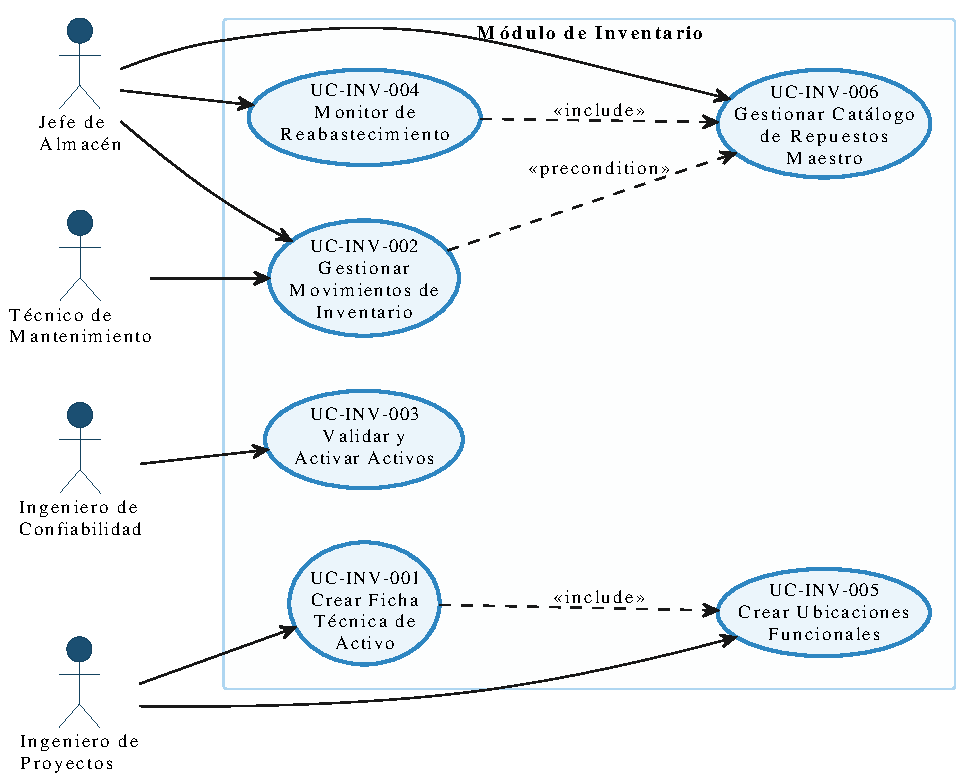
\includegraphics[width=0.85\textwidth]{assets/Diagrama-UC-INV.pdf}
\caption{Diagrama de Casos de Uso - Gestión de Recursos e Inventario}\end{figure}

\noindent\textbf{Ficha de Caso de Uso: UC-INV-002 - Gestión de Movimientos de Inventario}
\footnotesize\setlength{\tabcolsep}{4pt}\renewcommand{\arraystretch}{1.2}
\rowcolors{2}{tableBlue}{white}\begin{longtable}{>{\raggedright\arraybackslash}p{0.21\textwidth} >{\raggedright\arraybackslash}p{0.74\textwidth}} \toprule
\textbf{Actor Principal} & Jefe de Almacén \\
\textbf{Actores Secundarios} & Técnico de Mantenimiento (solicitante), Contabilidad (notificado) \\
\textbf{Descripción} & Permite registrar entradas, salidas y devoluciones de material con validación de stock disponible, trazabilidad completa y afectación financiera según prácticas Wireman Vol 2. \\
\textbf{Precondiciones} & \parbox[t]{\linewidth}{\vspace{2pt} \begin{itemize}[leftmargin=1.5em, nosep, topsep=0pt]
\item El usuario está autenticado con rol ``Jefe de Almacén''
\item El repuesto existe en el catálogo de repuestos maestro
\item La OT asociada (si aplica) está registrada y activa
\end{itemize} \vspace{2pt}} \\
\textbf{Flujo Principal} & \parbox[t]{\linewidth}{\vspace{2pt} \begin{enumerate}[leftmargin=1.5em, nosep, topsep=0pt]
\item El Jefe de Almacén ingresa al módulo de Movimientos y selecciona el tipo de movimiento: ``Entrada'', ``Salida'' o ``Devolución''.
\item El Sistema muestra el formulario correspondiente con campos obligatorios (FR-125 a FR-128).
\item El Jefe de Almacén selecciona el repuesto, ingresa la cantidad y confirma la operación.
\item El Sistema valida el stock disponible y las reglas de negocio (FR-126).
\item El Sistema registra el movimiento con su tipo y deja evidencia trazable del evento (FR-125 a FR-128, [TR-001]).
\item El Sistema actualiza los niveles de inventario y el saldo disponible (FR-126).
\item El Sistema comunica la confirmación: ``Movimiento registrado exitosamente''.
\end{enumerate} \vspace{2pt}} \\
\textbf{Flujos Alternativos} & \parbox[t]{\linewidth}{\vspace{2pt} \vspace{4pt}\noindent\textbf{AF-001: Stock Insuficiente para Salida}
\newline
En el paso 4, si el stock disponible es menor a la cantidad solicitada:
\begin{enumerate}[leftmargin=1.5em, nosep, topsep=0pt]
\item El Sistema bloquea la operación (FR-126).
\item El Sistema muestra mensaje: ``Stock insuficiente. Disponible: [X]. Requiere Orden de Compra''.
\item El flujo regresa al paso 2.
\end{enumerate}
\vspace{4pt}\noindent\textbf{AF-002: Devolución supera el máximo permitido}
\newline
En el paso 4, si la devolución supera el nivel máximo:
\begin{enumerate}[leftmargin=1.5em, nosep, topsep=0pt]
\item El Sistema acepta la devolución y registra alerta preventiva (FR-129).
\item El Sistema muestra advertencia de sobre-stock.
\item El flujo continúa en el paso 5.
\end{enumerate}
\vspace{4pt}\noindent\textbf{AF-003: Movimiento con OT no válida}
\newline
En el paso 3, si la OT asociada no está activa:
\begin{enumerate}[leftmargin=1.5em, nosep, topsep=0pt]
\item El Sistema bloquea la operación y solicita corrección (FR-127).
\item El flujo regresa al paso 2.
\end{enumerate} \vspace{2pt}} \\
\textbf{Postcondiciones} & \parbox[t]{\linewidth}{\vspace{2pt} \begin{itemize}[leftmargin=1.5em, nosep, topsep=0pt]
\item El movimiento queda registrado con trazabilidad completa
\item Los niveles de inventario quedan actualizados
\item El evento queda auditado de forma inmutable [TR-001]
\end{itemize} \vspace{2pt}} \\
\textbf{Requisitos} & FR-125 a FR-131 [TR-001] \\ \bottomrule
\end{longtable}\normalsize\vspace{1em}
\noindent\textbf{Ficha de Caso de Uso: UC-INV-006 - Gestión de Catálogo de Repuestos Maestro}
\footnotesize\setlength{\tabcolsep}{4pt}\renewcommand{\arraystretch}{1.2}
\rowcolors{2}{tableBlue}{white}\begin{longtable}{>{\raggedright\arraybackslash}p{0.21\textwidth} >{\raggedright\arraybackslash}p{0.74\textwidth}} \toprule
\textbf{Actor Principal} & Jefe de Almacén \\
\textbf{Actores Secundarios} & Auditor (consulta) \\
\textbf{Descripción} & Permite crear y mantener el catálogo maestro de repuestos con clasificación por commodity, validación de duplicados y reglas por tipo de inventario. \\
\textbf{Precondiciones} & \parbox[t]{\linewidth}{\vspace{2pt} \begin{itemize}[leftmargin=1.5em, nosep, topsep=0pt]
\item El usuario está autenticado con rol autorizado
\item La taxonomía de commodity está definida
\end{itemize} \vspace{2pt}} \\
\textbf{Flujo Principal} & \parbox[t]{\linewidth}{\vspace{2pt} \begin{enumerate}[leftmargin=1.5em, nosep, topsep=0pt]
\item El Jefe de Almacén accede al módulo del Catálogo de Repuestos Maestro y selecciona ``Nuevo Repuesto''.
\item El Sistema muestra formulario con campos obligatorios de clasificación y control (FR-170).
\item El Jefe de Almacén ingresa SKU, descripción, fabricante, commodity, clasificación ABC y tipo de inventario.
\item El Sistema valida unicidad del SKU y detecta posibles duplicados (FR-170, FR-171).
\item El Sistema confirma la clasificación y reglas aplicables según tipo (Stock/Direct Purchase) (FR-173).
\item El Jefe de Almacén guarda el repuesto.
\item El Sistema registra el nuevo repuesto y deja auditoría inmutable (FR-174, [TR-001]).
\item El Sistema comunica la confirmación: ``Repuesto creado exitosamente''.
\end{enumerate} \vspace{2pt}} \\
\textbf{Flujos Alternativos} & \parbox[t]{\linewidth}{\vspace{2pt} \vspace{4pt}\noindent\textbf{AF-001: Duplicado Potencial Detectado}
\newline
En el paso 4, si existe un repuesto similar:
\begin{enumerate}[leftmargin=1.5em, nosep, topsep=0pt]
\item El Sistema muestra advertencia con coincidencias (FR-171).
\item El Jefe de Almacén decide reutilizar el existente o crear nuevo.
\item El flujo continúa en el paso 6.
\end{enumerate}
\vspace{4pt}\noindent\textbf{AF-002: Tipo Direct Purchase}
\newline
En el paso 5, si el tipo es ``Direct Purchase'':
\begin{enumerate}[leftmargin=1.5em, nosep, topsep=0pt]
\item El Sistema oculta campos de stock y muestra mensaje informativo (FR-173).
\item El flujo continúa en el paso 6.
\end{enumerate} \vspace{2pt}} \\
\textbf{Postcondiciones} & \parbox[t]{\linewidth}{\vspace{2pt} \begin{itemize}[leftmargin=1.5em, nosep, topsep=0pt]
\item El repuesto queda registrado en el catálogo maestro
\item La clasificación ABC y commodity quedan disponibles para uso operativo
\item El evento queda auditado de forma inmutable [TR-001]
\end{itemize} \vspace{2pt}} \\
\textbf{Requisitos} & FR-170 a FR-176 [TR-001] \\ \bottomrule
\end{longtable}\normalsize\vspace{1em}